\chapter{Parameter and table choice}
\label{ch:param}
For the Time-Memory trade-off attack to viable, the right set of
parameters and the right table choice is of huge importance. In this
attack we would ideally want to perform the online phase of the  attack on a modern
high-end laptop/desktop machine. For this to be possible, the right
trade-off between time and memory is needed. For an attack on the
cipher with \code{64-bit} key size, we know a large table is required. But if
we want to make it possible to perform the attack on a (heavily
upgraded) consumer
machine, we need to set an upper bound for the maximal memory
usage. In our attack, we set an upper bound of memory usage to around
\code{8TB} of tables. We see this as a possible amount of storage if a
consumer machine with a TMTO-attack in mind was to be build. 

Knowing this and taking the theory behind the
TMTO-attack\footnote{Chapter \ref{ch:tmto}} into consideration, we
have to argue that this upper bound is required to be hit. For every
trade-off we take towards lower memory usage, the online phase of the
attacks will take a hit. 

Another thing to take into consideration when analyzing the parameter
choice and time consumption of the different phases is the table lookup
time. Since generated TMTO tables for a \code{64-bit} key size will
always be larger than a given built machines amount of RAM, look-ups are
done directly on a HDD or SSD. Estimates of how much time is required
for each lookup in a table is hard to do, but will be further analyzed
in SOMEWHERE? 

As for success probability of the 
the different attacks, we went with $P = 73\%$ as an acceptable
success rate.
We witnessed that for a probability of above $73\%$ the increase,
in both pre-computational cost and the time of the online phase, would
make our initial idea of running the attack on a consumer made PC
unfeasible.

In the following sections we will go through our computations of
parameters for the different TMTO-attacks with these limits set.

\section{Hellman Table}

All calculations of parameters follows the theory provided in \ref{sec:hmtheory}.

\section{Distinguished Points Table}

All calculations of parameters follows the theory provided in \ref{sec:dptheory}.

\section{Rainbow Table}
For the Rainbow Table TMTO attack, we again set \code{8TB} as the
upper bound for memory consumption. 

All calculations of parameters follows the theory provided in
\ref{sec:raintheory}. 

In our calculations, we assume a sequential approach is done in the
pre-computational phase. This allows us to remove half of the memory
cost compared to storing both start point and end point.

Table \ref{tab:rainparam} shows the relation between \code{t} and
\code{m} in a Rainbow attack, when the success rate of $73\%$ is set\footnote{Tables for $P = 58\%, P = 73\%, P = 90\%$ and tables $l=1..3$ are generated and can be
found in Appendix \ref{sec:rainbowtab}.}. Figures \ref{fig:param73}
and \ref{fig:time73} shows the graphical representation of the table.

\begin{table}[H]
  \centering
  \text{\texttt{Success{ }={ }0.730000,{ }Rmsc{ }={ }1.849002,{ }l{ }={ }1,{ }Offline{ }phase{ }={ }2{\char`\^}64.886747}}
  \begin{tabular}{llll}
    m & t & M(TB) & T \\ \hline
    $2^{35.50}$ & $2^{29.39}$ & $0.39$ & $2^{56.58}$ \\
    $2^{36.00}$ & $2^{28.89}$ & $0.55$ & $2^{55.58}$ \\
    $2^{36.50}$ & $2^{28.39}$ & $0.78$ & $2^{54.58}$ \\
    $2^{37.00}$ & $2^{27.89}$ & $1.10$ & $2^{53.58}$ \\
    $2^{37.50}$ & $2^{27.39}$ & $1.55$ & $2^{52.58}$ \\
    $2^{38.00}$ & $2^{26.89}$ & $2.20$ & $2^{51.58}$ \\
    $2^{38.50}$ & $2^{26.39}$ & $3.11$ & $2^{50.58}$ \\
    $2^{39.00}$ & $2^{25.89}$ & $4.40$ & $2^{49.58}$ \\
    $2^{39.50}$ & $2^{25.39}$ & $6.22$ & $2^{48.58}$ \\
    $2^{40.00}$ & $2^{24.89}$ & $8.80$ & $2^{47.58}$ \\
  \end{tabular}
  \caption{Rainbow Parameters}
  \label{tab:rainparam}
\end{table}
\begin{figure}[H]
  \centering
  \begin{minipage}{.5\textwidth}
    \centering
    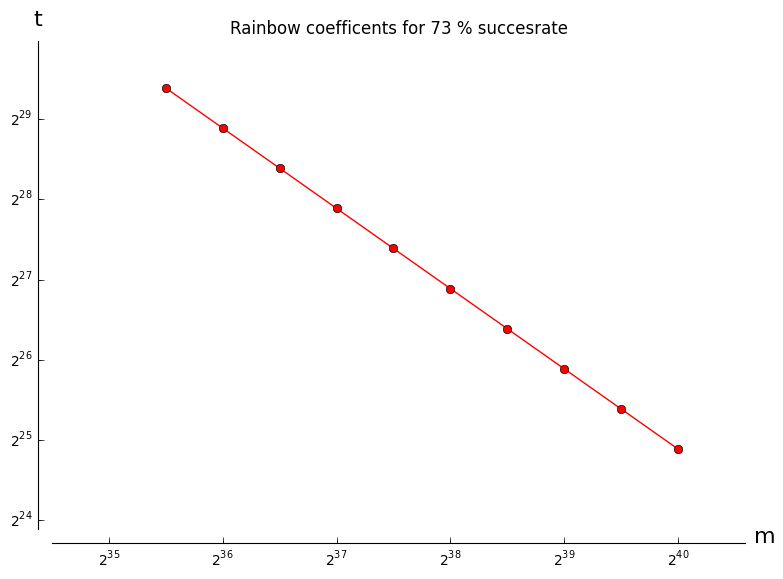
\includegraphics[scale=0.3]{figures/RainbowCoef73.png}
    \captionof{figure}{Rainbow Parameters 73\% success}
    \label{fig:param73}
  \end{minipage}%
  \begin{minipage}{.5\textwidth}
    \centering
    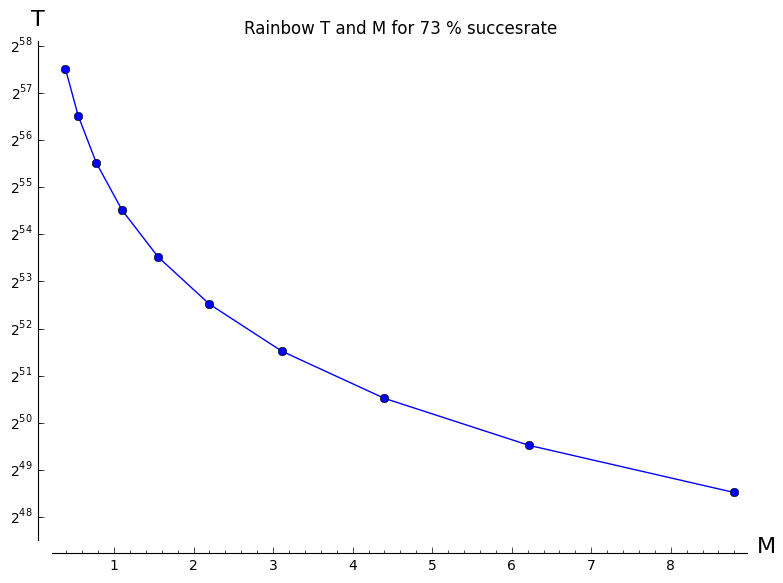
\includegraphics[scale=0.3]{figures/RainbowTime73.png}
    \captionof{figure}{Rainbow TMTO 73\% success}
    \label{fig:time73}
  \end{minipage}
\end{figure}

Looking at table \ref{tab:rainparam} and figures \ref{fig:param73}
and \ref{fig:time73}\footnote{See Appendix \ref{sec:rainbowgraphs} for
  full size graphs} while knowing that 

\newpage
\section{Comparison and choice of table}

%%% Local Variables:
%%% mode: latex
%%% TeX-master: "Thesis"
%%% End:
